\chapter{Reconstruction of physics objects}
    \label{chapter:ReconstructionOfObjects}

This chapter describes the reconstruction of the main physics objects that are relevant for the analysis presented in this Thesis.
The identification, reconstruction and calibration of electrons, muons, jets and missing transverse energy is discussed in detail.

\section{Electrons}
    \label{sec:ElectronReco}

In the following, the electron reconstruction and identification will be described.
The reconstruction step is used to define the electron candidates, while the identification selects electron samples with different purities.

\subsection{Electron reconstruction}
    \label{subsec:ElectronReconstruction}

The electron reconstruction can be divided into central and forward.
In the central region, $|\eta|<2.47$, the electron reconstruction starts from energy deposits (clusters) in the electromagnetic calorimeter that are associated to reconstructed tracks of charged particles in the Inner Detector.
The reconstruction of the electron clusters is based on a fixed-size sliding window algorithm \cite{Lampl:2008zz}.

The tracks are extrapolated from their last measurement point in the inner detector to the second layer of the EM calorimeter and the coordinates from the impact point are then compared to those of the seed cluster.
The cluster matching is performed if at least one track is matched to the seed cluster.
In the case where several tracks are matched to the same cluster, tracks with silicon hits are preferred and the one with the smallest $\Delta R$ distance to the seed cluster is chosen.

The four-momentum of the central electrons is computed using the information from both the final cluster and the best track matched to the original seed cluster.
While the energy is given entirely by the cluster energy, the $\eta$ and the $\phi$ directions are taken from the corresponding track parameters at the vertex.

In the forward region, $2.5 < |\eta| < 4.9$, there are no tracking detectors. Therefore, the electron candidates are reconstructed only from energy deposits in the calorimeters. These clusters are built using a topological clustering algorithm, that will be explained in Section~\ref{sec:JetReco}.

\subsection{Electron identification}
    \label{subsec:ElectronIdentification}

The electron identification aims to provide good separation between isolated electrons and jets faking electrons.
It consist of a cut-based selection on variables that use calorimeter, tracking and combined calorimeter and tracker information.
Three sets of reference selection criteria have been defined with increasing background rejection power: \textit{loose}, \textit{medium} and \textit{tight}, as described in Ref.~\cite{Aad:2011mk}.
The shower shape variables calculated in the second EM calorimeter layer and hadronic leakage variables are used in the loose selection.
These shower shape variables are binned in $\eta$ and $\met$, allowing a proper handling of correlations between variables and assuring the highest efficiency for a given jet rejection \cite{Aad:2014fxa}.
Cuts on the first EM calorimeter layer variables, track quality requirements and track-cluster matching are added in the medium selection.
Finally, in the tight selection, the track quality requirements are tightened.
For the analysis presented in this Thesis, only electrons following the \textit{medium} identification criteria are considered.


\subsection{Electron energy corrections}
    \label{subsec:ElectronEnergyCorrections}

The reconstructed electron energy in data is tuned to reproduce the $Z$ mass peak central value according to the $Z$ mass world average by applying extra corrections as a function of $|\eta|$ \cite{Aad:2011mk}:

\begin{equation}
E_{\text{corrected}} = \frac{E}{1+\alpha},
\label{eq:ElectronEnergyCalibration}
\end{equation}

\noindent where $\alpha$ measures the residual miscalibration. The values of $\alpha$ are within $\pm 2 \%$ in the barrel region and within $\pm 5 \%$ in the forward regions.
The calibrated electron energy scale is further validated with electron candidates from $J/\psi\rightarrow ee$ events in data, and determined with a precision of 0.3--1.6\% in the central region over $|\eta|<2.47$, for different $|\eta|$ values \cite{Aad:2014nim}.

\section{Muons}
    \label{sec:MuonReco}

This section presents the muon reconstruction and identification in ATLAS, which mainly relies on the information extracted from the Inner Detector and the Muon spectrometer. 


\subsection{Track reconstruction}
    \label{subsec:MuonTrackReconstruction}

The tracks of the muon candidates are reconstructed independently in the ID and the MS.
Hits in each station of the Muon Spectrometer are combined to build track segments up to $|\eta|<2.7$.
A similar approach is followed in the inner detector, where the pattern recognition uses space points from the pixel and SCT clusters to generate seeds, which are then extended into the TRT.

\subsection{Muon identification}
    \label{subsec:MuonIdentification}

In ATLAS, the muon identification is performed according to several reconstruction criteria, which leads to different muon ``types''.
These types are defined based on the available information from the ID, the MS and different calorimeter sub-detector systems~\cite{Aad:2014rra}:

\begin{itemize}
\item{Stand-alone (SA):} The muon trajectory is only reconstructed in the muon spectrometer. The direction of flight and the impact parameter of the muon at the interaction point are determined by extrapolating the spectrometer track back to the beam line.
\item{Combined muon (CB):} The momentum of the stand-alone muon is combined with the momentum measured in the ID, which also provides information about the impact parameter of the muon trajectory with respect to the primary vertex.
\item{Segment tagged (ST):} A trajectory in the inner detector is identified as a muon if the trajectory extrapolated to the muon spectrometer can be associated with straight track segments in the precision muon chambers.
\item{Calorimeter tagged (CaloTag):} A trajectory in the ID is identified as a muon if the associated energy depositions in the calorimeters is compatible with the hypothesis of a minimum ionizing particle.
\end{itemize}

The analysis described in this Thesis uses combined muons and segment tagged muons, reconstructed with the \textit{staco} reconstruction chain, as described in Ref.~\cite{Hassani:2007cy}.
Combined muons are the highest purity muon candidates.
Tagged muons give additional efficiency, as they can recover muons which did not cross enough precision chambers to allow an independent momentum measurement in the Muon Spectrometer.

The reconstructed muon momentum in data is tuned to reproduce the $Z$ and $J/\Psi$ masses as it was done for electrons, and needs to be studied separately in the ID and the MS.
The dimuon invariant mass resolution of combined muons is found to vary between 2 and 3 GeV, as a function of $|\eta|$. 


\section{Jets}
    \label{sec:JetReco}

In hard interactions, quarks and gluons result in showers of collimated particles, called \textit{jets}.
A well-defined jet algorithm is needed in order to establish a correspondence between observables at partonic, hadronic and detector level.
Jets are reconstructed using the $\akt$ algorithm, described in the following.


\subsection{Jet finding algorithm}
    \label{subsec:JetClusteringAlgorithm}


The $\akt$~\cite{Cacciari:2008gp} is a sequential recombination algorithm, and is the default jet finding algorithm in the LHC experiments.
It starts from an input list of four-vectors, which can be either particles from the $\pp$ interactions simulated in the MC with a lifetime longer than 10~ps (\emph{truth constituents}), reconstructed charged particle tracks associated with the reconstructed primary collision vertex (\emph{track constituents}), or energy depositions in the ATLAS calorimeters (\emph{calorimeter constituents}).
The jet reconstruction in ATLAS is summarized in Figure~\ref{fig:JetReconstructionOverview}.

\begin{figure}[!ht]
  \begin{center}
    \mbox{
      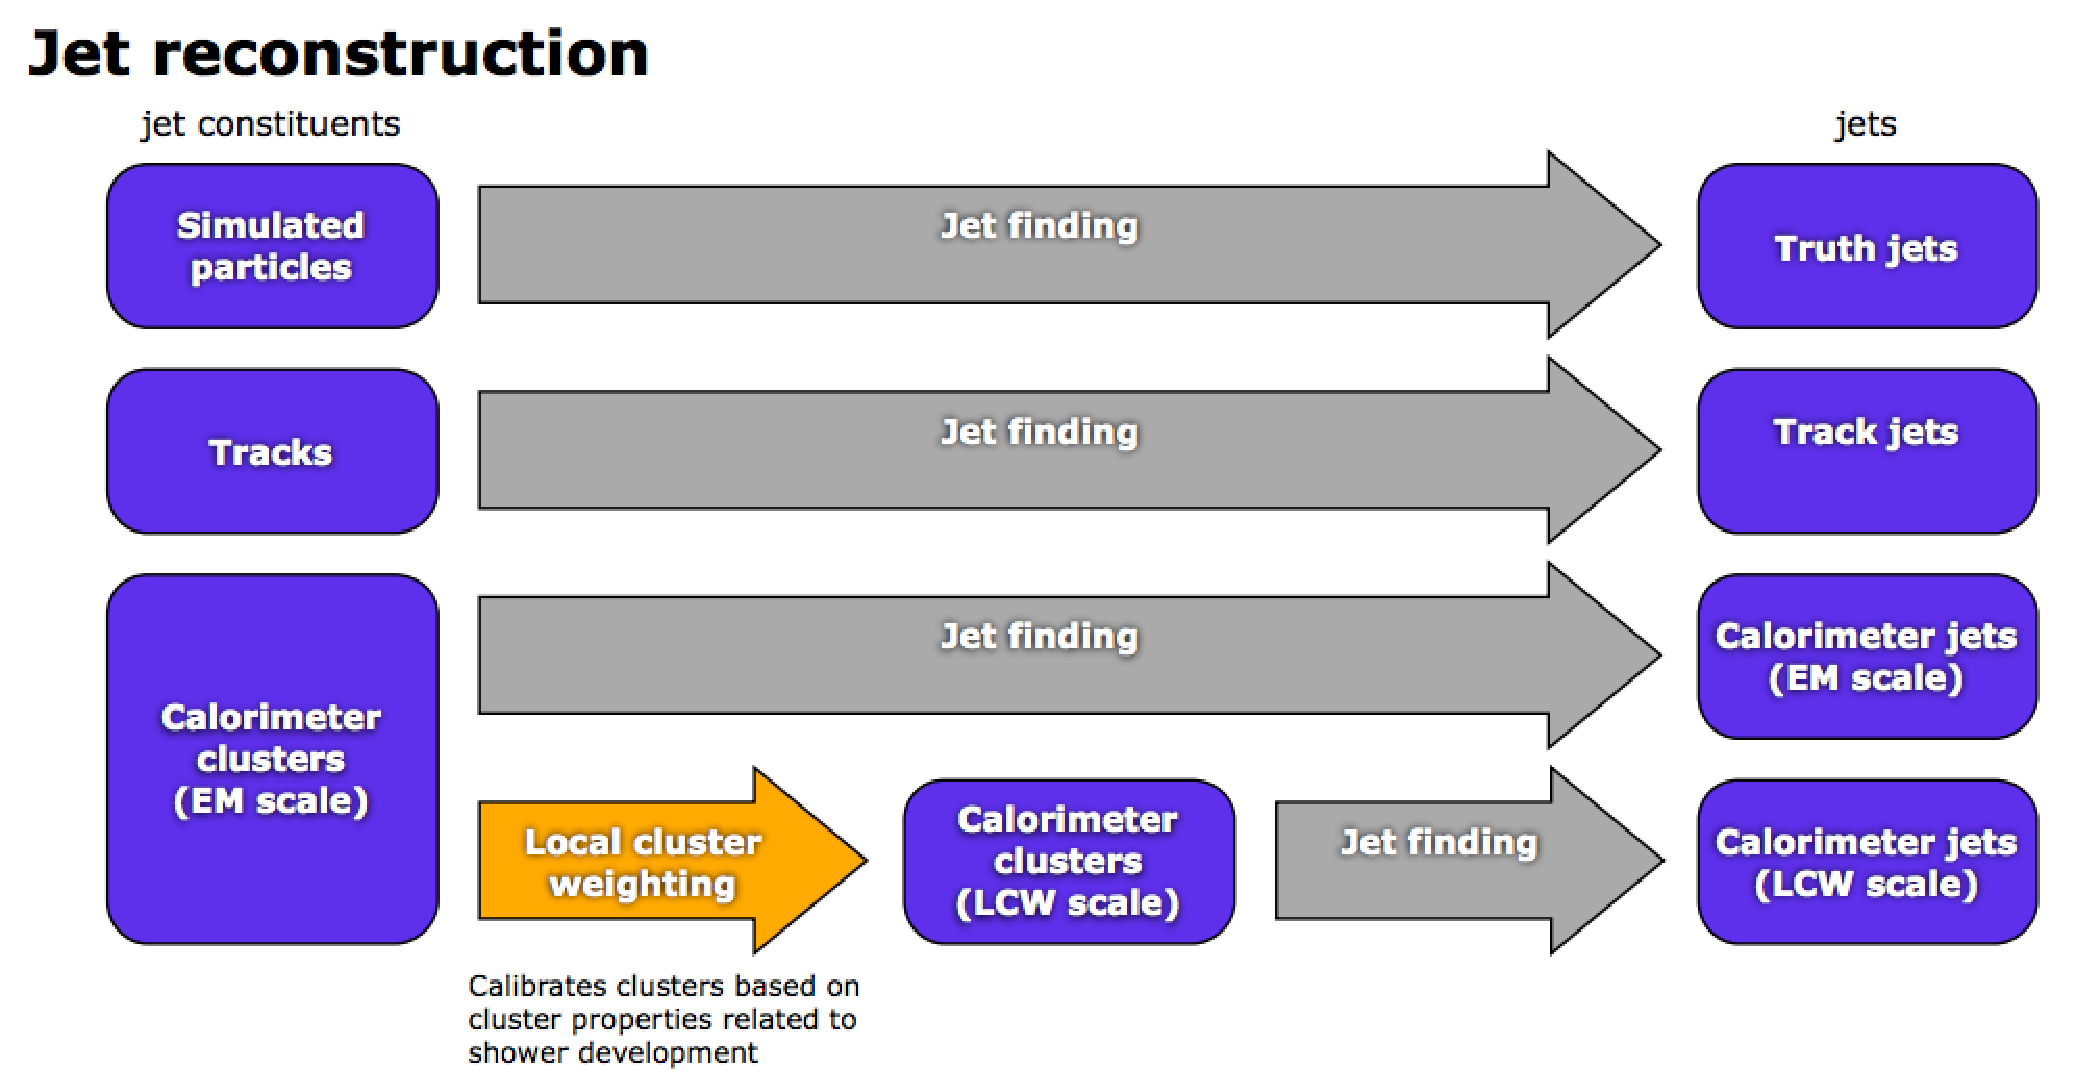
\includegraphics[width=0.995\textwidth]{ObjectReconstruction/Figures/JetReconstructionOverview.eps}
    }
  \end{center}
  \caption[Overview of the ATLAS jet reconstruction.]{Overview of the ATLAS jet reconstruction~\cite{Aad:2014bia}.}
  \label{fig:JetReconstructionOverview}
\end{figure}

For all the input constituents, the $\akt$ algorithm computes the quantities:

\begin{subequations}
    \begin{equation}
        d_{ij} = \min\left( \frac{1}{k_{ti}^{2}}, \frac{1}{k_{tj}^{2}} \right) \frac{\Delta R_{ij}^{2}}{R^2}
        \label{eq:AntiKt_dij}
    \end{equation}
    \begin{equation}
        d_{iB} = \frac{1}{k_{ti}^{2}},
        \label{eq:AntiKt_diB}
    \end{equation}
\end{subequations}

\noindent where $\Delta R_{ij}^{2} = (\eta_i - \eta_j)^2 + (\phi_i - \phi_j)^2$, $R$ is a parameter of the algorithm that approximately controls the size of the jet and $k_{ti}$ is the transverse momentum of the constituent $i$.
Here, $d_{ij}$ is the ``distance'' between the constituents $i$ and $j$, while $d_{iB}$ is the distance between the constituent $i$ and the beam, introduced to separate constituents coming from the interactions from proton remnants.

The $\akt$ jet clustering algorithm proceeds by identifying the smallest of the distances. 
If the smallest distance is a $d_{ij}$, it recombines the entities $i$ and $j$, while if the smallest distance is $d_{iB}$, the algorithm calls $i$ a jet and removes it from the list of entities.
The method used to recombine the different constituents is called \emph{recombination scheme}.
In ATLAS, the $E$-scheme is used, in which the four-momentum of the recombined object is defined by the vectorial sum of the four-momenta of its constituents.
After recombination, the distances are recalculated with the remaining objects, and the procedure repeated until no entities are left.

The $\akt$ algorithm defines jets with a well-defined conical shape, thus allowing robust pileup corrections.
Jets are defined with a minimum transverse momentum threshold $p_T^{\text{jet}}$, used as a scale to separate soft from hard interactions.
Figure \ref{fig:JetTopoClusterAntiKt} (left) illustrates the clustering of hard and soft particles into jets when the $\akt$ algorithm is applied.

\begin{figure}[!ht]
  \begin{center}
    \mbox{
      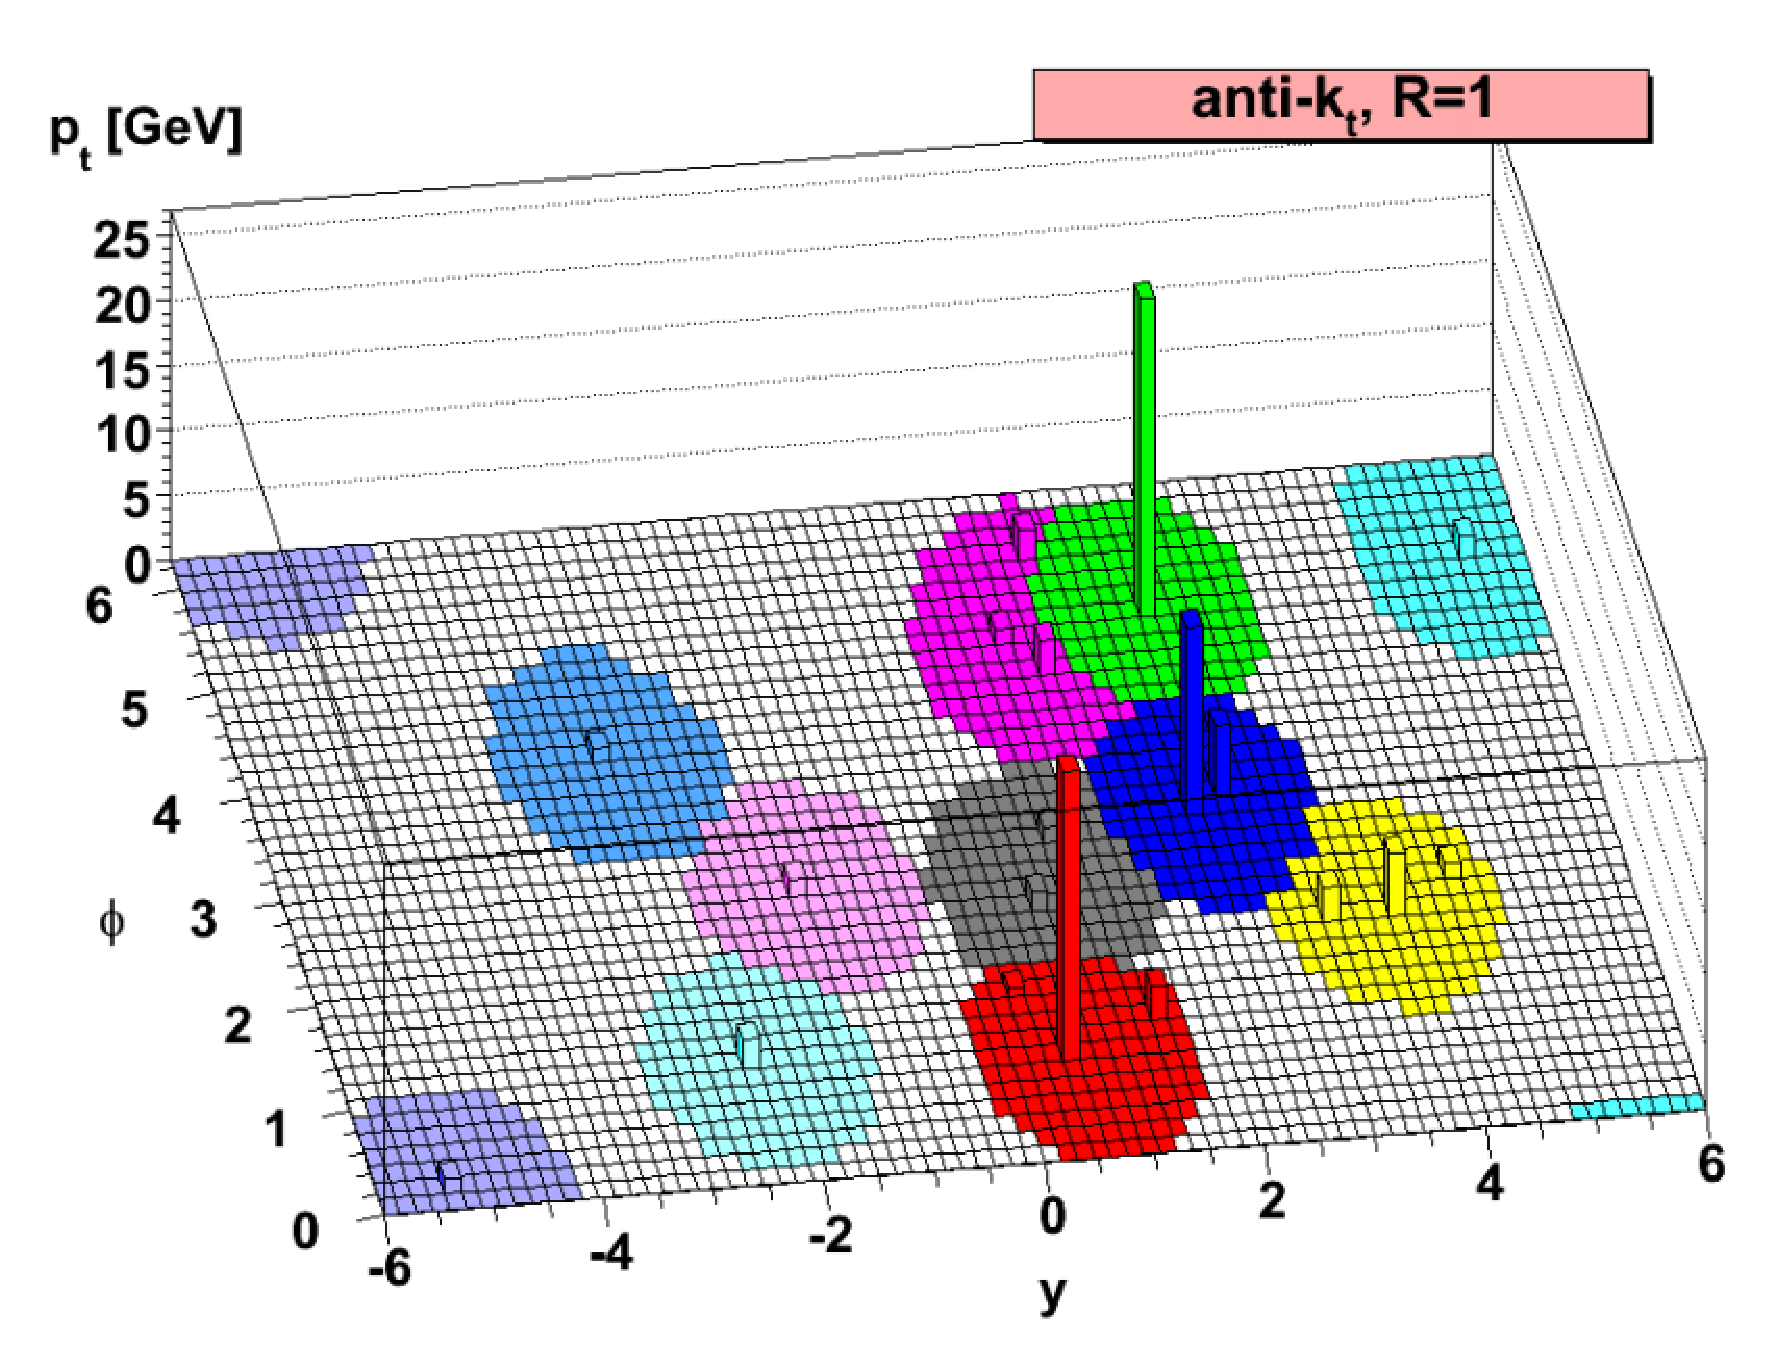
\includegraphics[width=0.495\textwidth]{ObjectReconstruction/Figures/JetAntiKt.eps}
      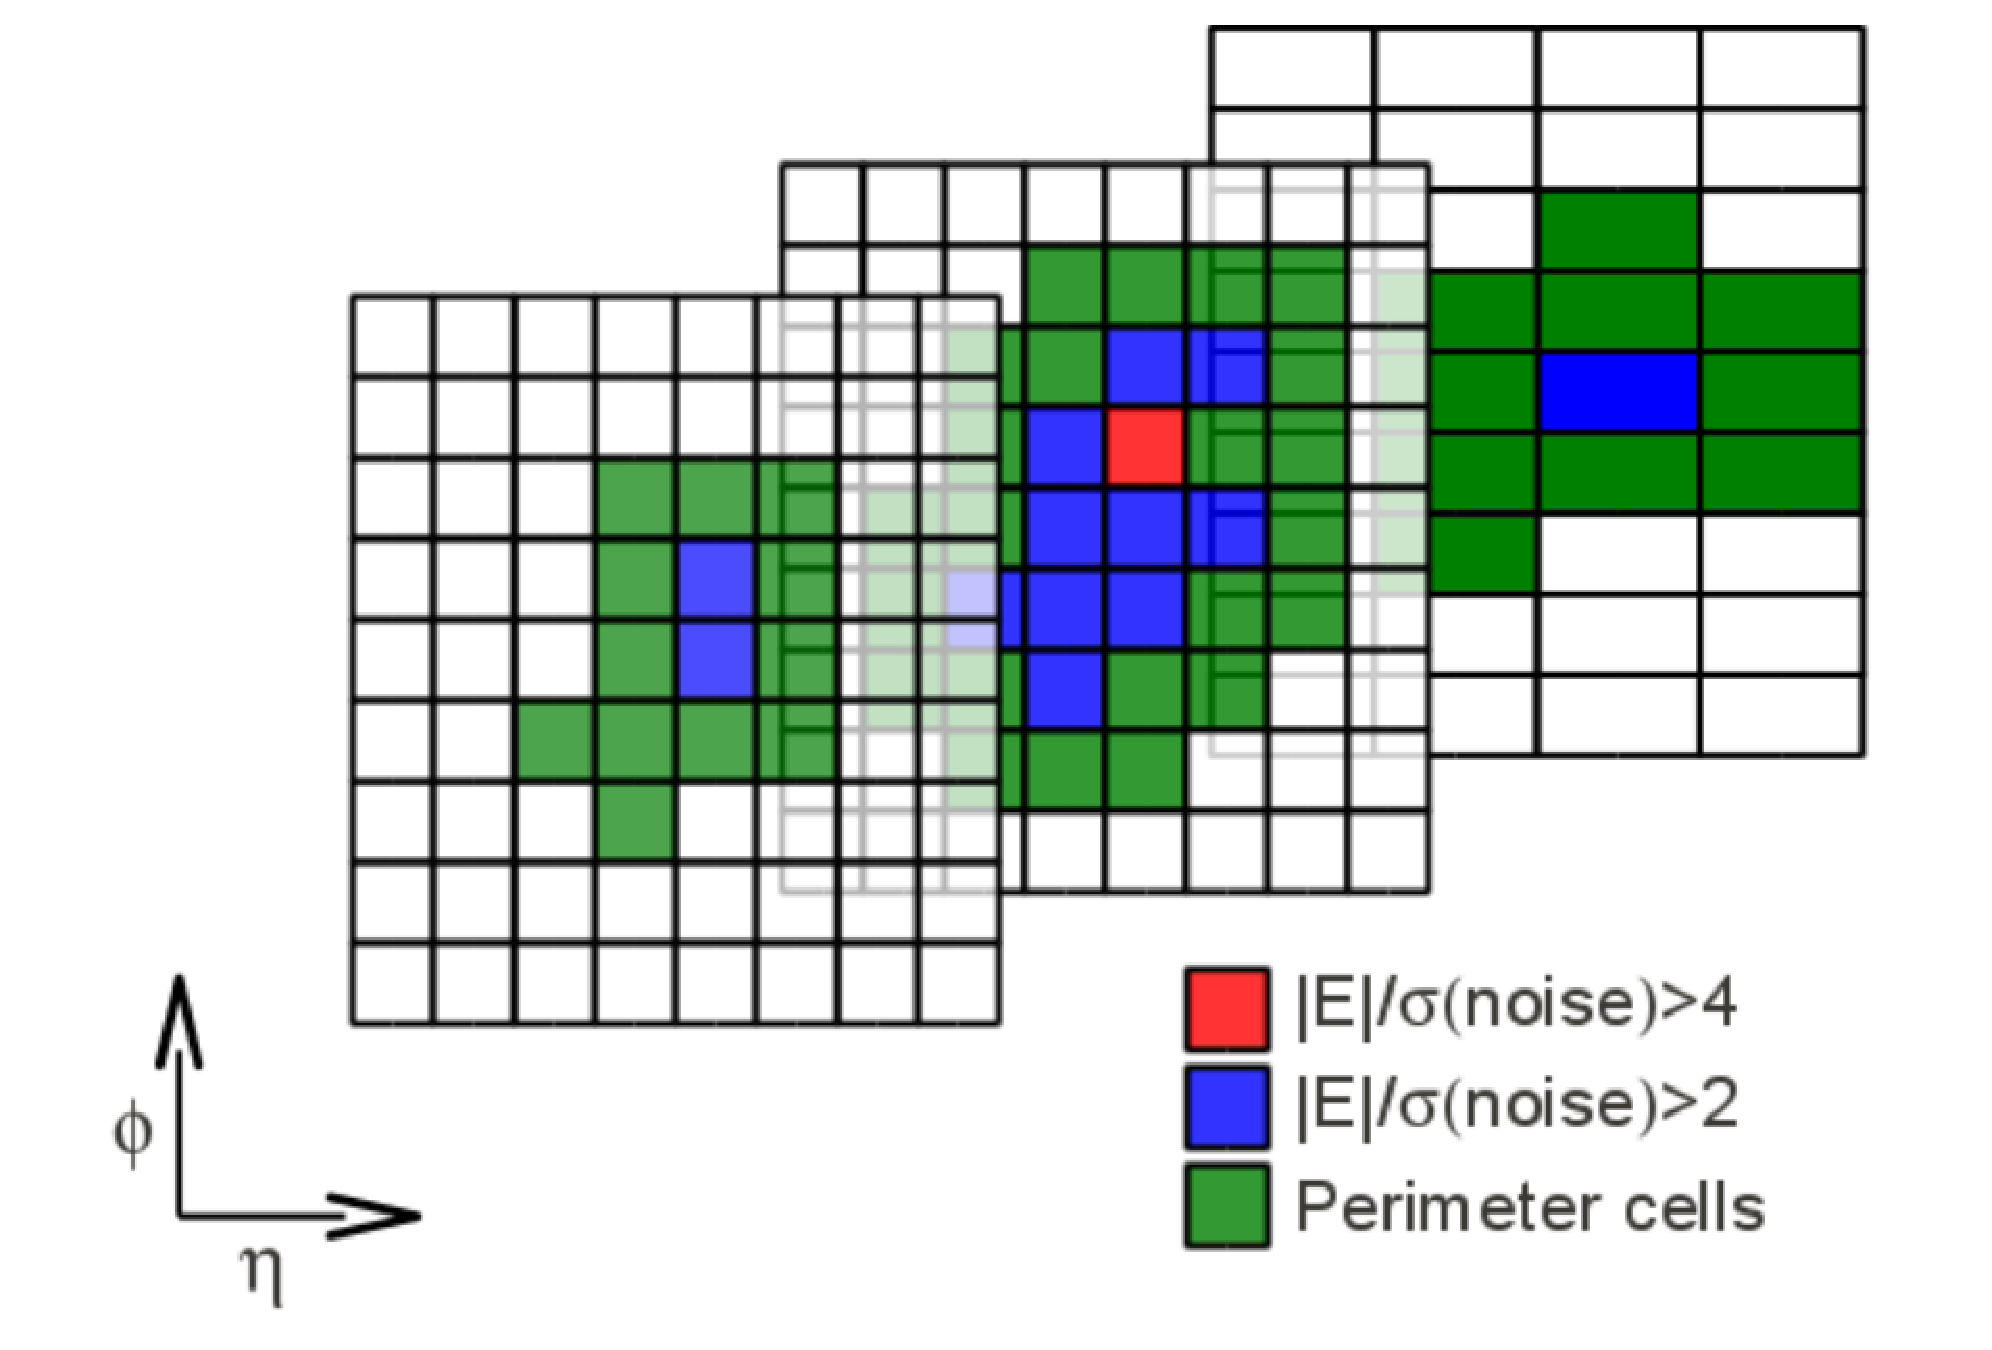
\includegraphics[width=0.495\textwidth]{ObjectReconstruction/Figures/JetClusterFormation.eps}
    }
  \end{center}
  \caption[Illustration of the ``active'' catchment area of the $\akt$ algorithm (left). Topo-cluster formation in the three hadronic layers in the barrel and $\akt$ jet algorithm representation (right).]{
  Illustration of the clustering of the jets with the $\akt$ algorithm~\protect\cite{Cacciari:2008gp} (left).
    Grid representing calorimeter cells, showing topo-cluster formation in the three hadronic layers in the barrel (right). 
  }
  \label{fig:JetTopoClusterAntiKt}
\end{figure}



\subsection{Cluster formation}
    \label{subsec:JetClusterFormation}

The calorimeter constituents mentioned in the previous section are reconstructed with the topological clustering (topo-cluster) algorithm \cite{Lampl:2008zz}.
This algorithm, reconstructs 3-dimensional clusters, and is designed to follow the shower development of a single particle interacting with the calorimeter, taking advantage of the calorimeters fine granularity.

Figure \ref{fig:JetTopoClusterAntiKt} (right) shows a schema of a topological cluster formation.
Seed cells are built by selecting cells with a significant signal to noise ratio of $|S/N|\geq 4$.
The noise is defined as the expected RMS of the electronics noise for the current gain and conditions plus the contribution of pileup added in quadrature.
Neighboring cells in the 3 dimensions are then added to the cluster if their signal to noise ratio is $|S/N|\geq 2$.
Finally, cells with $|S/N|\geq 0$ in the perimeter are added to the cluster, to ensure that the tails of showers are not discarded, while the higher thresholds for seeds and neighbors effectively suppress both electronics and pile-up noise.
In case of particles leading to overlapping showers they can still be separated if they form local maxima in the calorimeter.
Topo-clusters are defined to be massless and represent three dimensional energy blobs in the calorimeter.



\subsection{Jet calibration}
    \label{subsec:JetCalibration}

Topo-clusters are initially reconstructed at the EM scale, which correctly measures the energy in the calorimeter deposited by particles produced in an electromagnetic shower.
These clusters then need to be recalibrated to correctly measure the energy deposited by particles produced in an hadronic shower.
This is done with the local cell signal weighting (LCW).
LCW first classifies topo-clusters as either electromagnetic or hadronic based on the measured energy density and the longitudinal shower depth.
Then, energy corrections are derived according to this classification from single charged and neutral pion MC simulations.
Further dedicated corrections address effects of calorimeter non-compensation, signal losses due to noise threshold effects and energy loss in non instrumented regions of the detector close to the cluster.

Figure~\ref{fig:JetCalibrationFlow} shows an overview of the ATLAS calibration scheme for calorimeter jets, which restores the jet energy scale to that corresponding to particle-level jets before detector effects.
It consists of four steps, briefly discussed below:

\begin{figure}[!ht]
  \begin{center}
    \mbox{
      
\includegraphics[width=0.995\textwidth]{ObjectReconstruction/Figures/JetCalibrationFlow.eps}
    }
  \end{center}
  \caption{Overview of the ATLAS jet calibration~\cite{Aad:2014bia}.}
  \label{fig:JetCalibrationFlow}
\end{figure}


\begin{enumerate}
\item{\textbf{Pileup correction:}} The jets formed from topoclusters at the EM or LCW scale are first corrected to account for the energy offset due to pileup. This procedure is explained in detail in Section \ref{subsubsec:JetPileupCorrections}.

\item{\textbf{Origin correction:}} A correction to the calorimeter jet direction is applied to make that the jet points back to the primary event vertex instead of the center of the nominal ATLAS detector. 
Thereafter, the kinematic observables of each topo-cluster are recalculated.
This correction improves the angular resolution and results in a small improvement in the jet $\pt$ response.
The energy of the jet remains unchanged. 

\item{\textbf{Jet calibration based on MC simulation:}} The jet energy calibration is derived from simulation, by relating the reconstructed jet energy to the particle-level jet energy. 
The jet energy calibration is discussed in detail in Section \ref{subsubsec:JetEnergyCalibration}.

\item{\textbf{Residual \emph{in-situ} corrections:}} This correction assesses the differences between the data and the MC simulations.
It is applied as the last step to the jets reconstructed in data, and is explained in detail in Section \ref{subsubsec:JetResidualCalibration}.
\end{enumerate}


\subsubsection{Pileup corrections}
    \label{subsubsec:JetPileupCorrections}

The correction applied to jets to account for the energy offset introduced by the several interactions per bunch crossing in ATLAS is discussed below.
The mean number of inelastic $\pp$ interactions per bunch crossing, $\averageIntXing$, is related to the instantaneous luminosity, $\InstLumi$, by Equation~\ref{LumiDefinition}, which can be re-written as

\begin{equation}
\averageIntXing = \frac{\InstLumi \times \sigma_{\text{inel.}}}{n_b \times f_r}.
\label{eq:intPerXing}
\end{equation}

The instantaneous luminosity in 2012 reached values as high as $\unit[7.7\times10^{33}]{cm^{-2} s^{-1}}$, meaning that the average pileup activity in 2012 was $\averageIntXing \approx 20.7$.

The presence of these additional interactions per bunch crossing can effect the data-taking in two different ways:

\begin{itemize}
\item{\emph{In-time} pileup: } additional signals in the calorimeters can be produced due to the presence of additional interactions in the same bunch crossing as the triggered event.
\item{\emph{Out-of-time} pileup:} further signal modulation in the calorimeters from multiple interactions in surrounding bunch crossings.
\end{itemize}

In order to account for these effects, corrections of the jet transverse momentum that inherently accommodates jet-by-jet variations in pileup sensitivity as well as event-by-event fluctuations in pileup activity are applied according to Equation \ref{eq:JetPileupCorrection},

\begin{equation}
\pt^{\text{jet, corr}} = \pt^{\text{jet}} - \rho \cdot A - \text{Residuals}(N_{\text{PV}}-1, \averageIntXing, \pt)
\label{eq:JetPileupCorrection}
\end{equation}

\noindent where $\rho$ is the median $\pt$ density which provides a direct estimate of the global pileup activity in any event, and $A$ is the jet area, which provides an estimate of a jet's sensitivity to pileup. By the multiplication of these two quantities, an estimate of the effect of the in-time pileup on the jet is obtained.
However, Ref.~\cite{TheATLAScollaboration:2013pia} shows that the effects of pileup in the forward region are not well described by $\rho$. 
After subtracting $\rho \cdot A$ from the jet $\pt$, an additional subtraction of a residual term is needed.
This residual term provides, as a function of the jet $\pt$, corrections for in-time and out-of-time pileup effects.
For this reason, the residual term is proportional to the number of reconstructed pileup vertices, $N_{\text{PV}}-1$, and to $\averageIntXing$, respectively.
Figure \ref{fig:JetPileupCorrection} shows the dependence of the reconstructed jet $\pt$ on in-time pileup (left) and out-of-time pileup (right) at various correction stages for different $|\eta|$.

\begin{figure}[!ht]
  \begin{center}
    \mbox{
      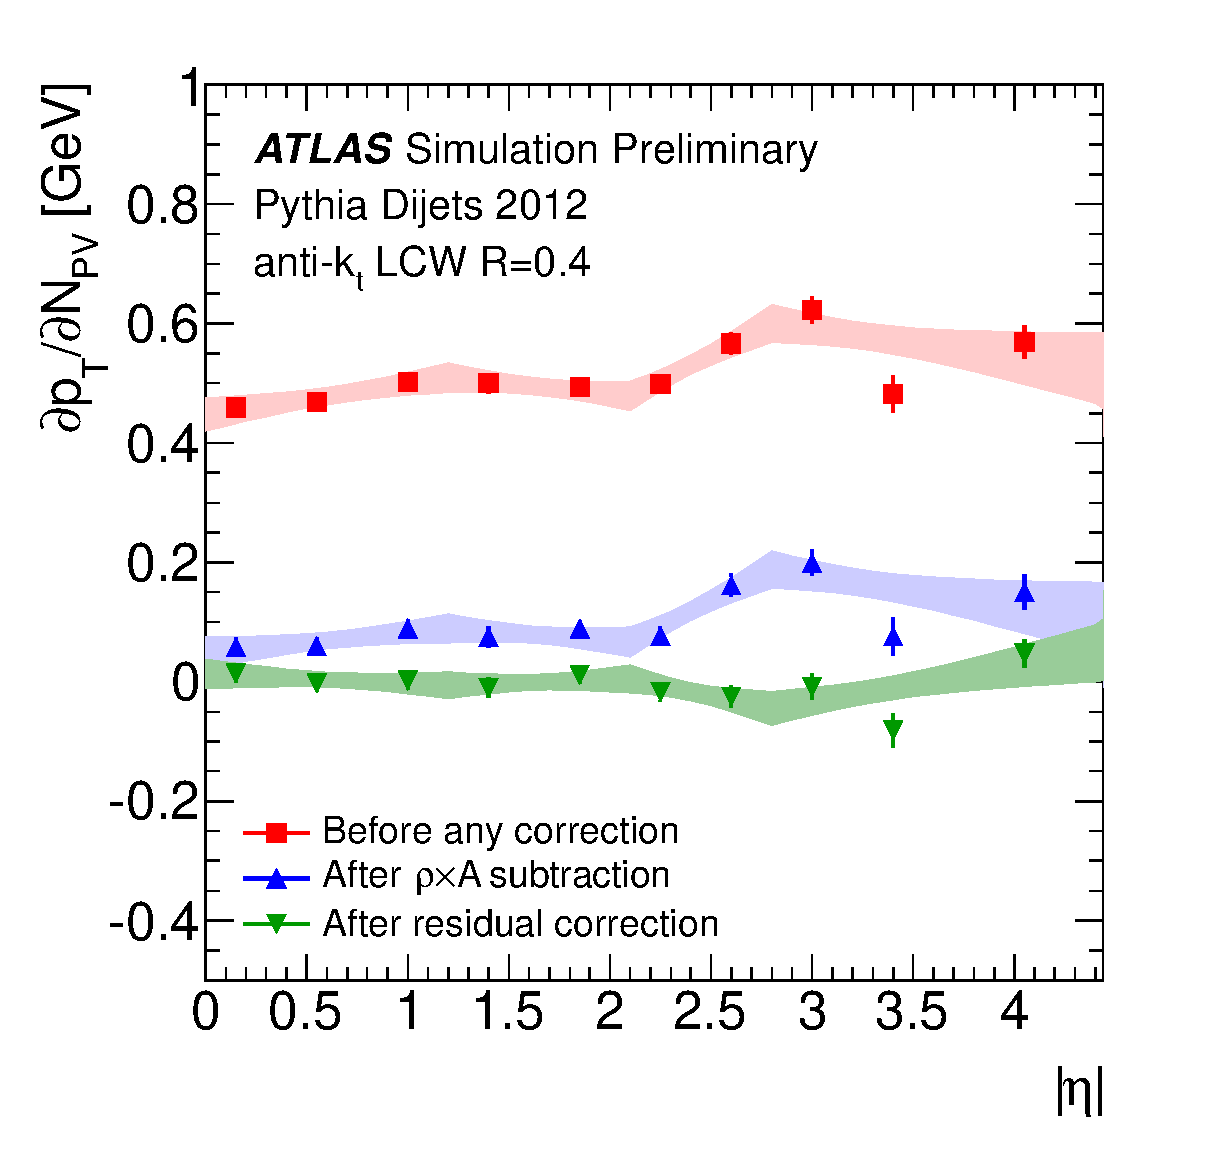
\includegraphics[width=0.495\textwidth]{ObjectReconstruction/Figures/JetPileupCorrNPV.eps}
      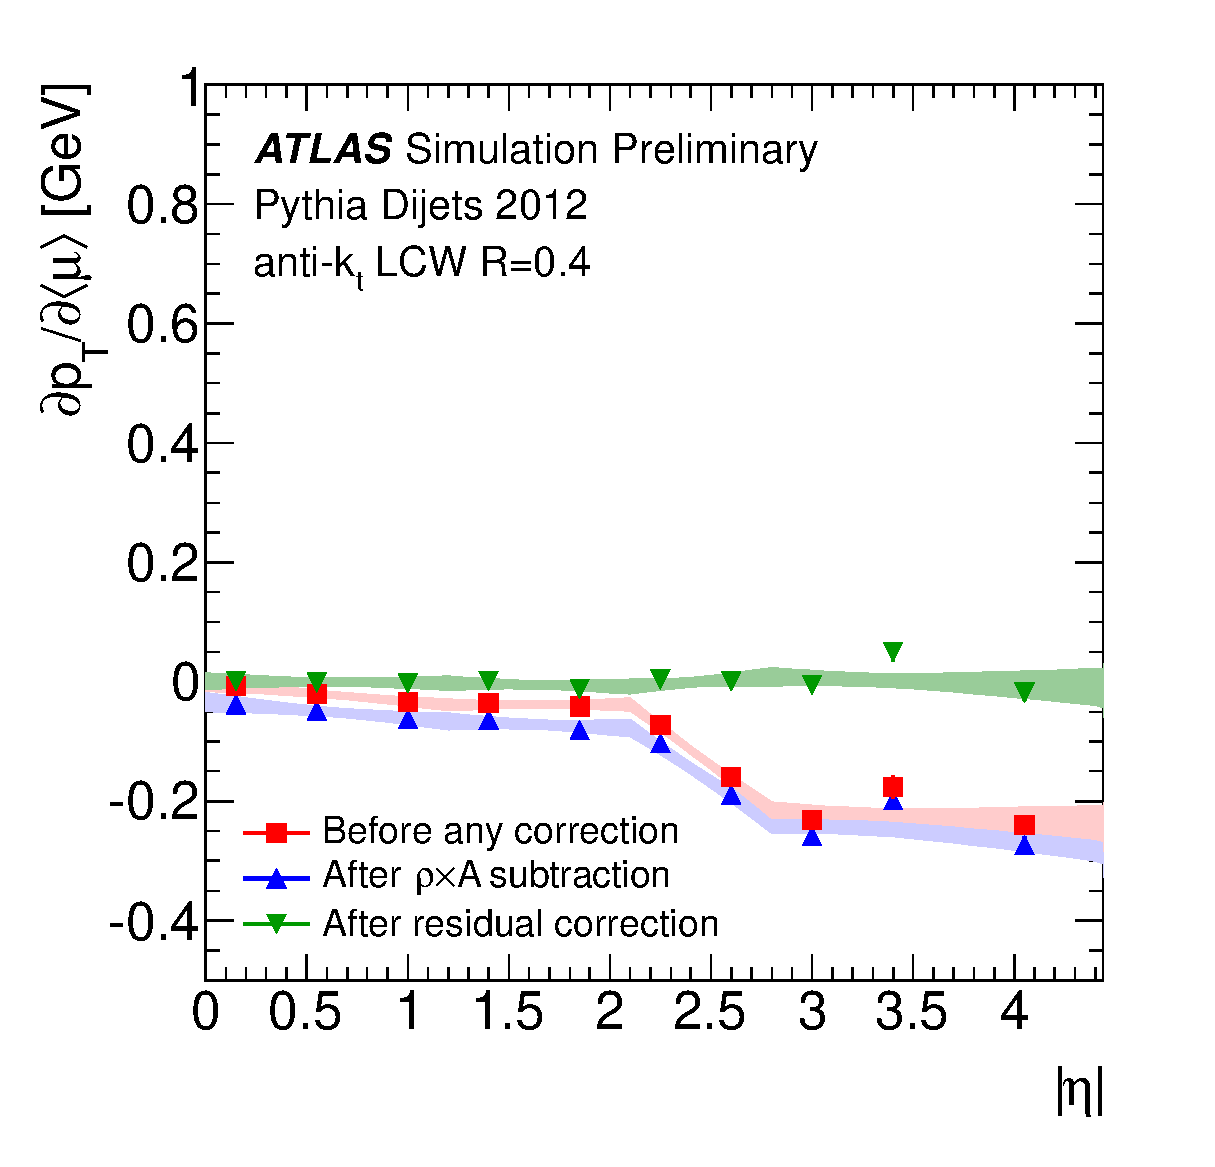
\includegraphics[width=0.495\textwidth]{ObjectReconstruction/Figures/JetPileupCorrMu.eps}
    }
  \end{center}
  \caption[Dependence of the reconstructed jet $\pt$ on in-time pileup and out-of-time pileup at various correction stages.]{Dependence of the reconstructed jet $\pt$ on in-time pileup (left) and out-of-time pileup (right) at various correction stages~\protect\cite{TheATLAScollaboration:2013pia}.}
  \label{fig:JetPileupCorrection}
\end{figure}

The fluctuations due to pileup effects in the energy of the jets with energies around the $\pt$ threshold or the reconstruction of jets coming from other pileup interactions, can increase the jet multiplicity of an event.
In order to reject these jets, information from the tracks associated to each jet is used.
The jet vertex fraction (JVF) is a variable aiming to identify the vertex from which a jet is originated. 
A schematic representation of the JVF principle is shown in Figure \ref{fig:JetPileup} (left).
It is calculated as the ratio of the sum of transverse momentum of matched tracks that originate from a chosen PV to the sum of transverse momentum of all matched tracks in the jet, independently of their origin. 
JVF is defined for each jet with respect to each PV, and therefore for a given jet $i$, its JVF with respect to the primary vertex $j$, PV$_j$, is given by:

\begin{equation}
\text{JVF}(\text{jet}_i, \text{PV}_j) = \frac{\sum_{k=1}^{N_\text{tracks}}{\pt(\text{track}_{k}^{\text{jet}_i}, \text{PV}_j) }}{ \sum_{n=1}^{N_\text{PV}}{\sum_{l=1}^{N_\text{tracks}}{\pt(\text{track}_{l}^{\text{jet}_i}, \text{PV}_n)} }}.
\label{eq:JetJVFDefinition}
\end{equation}

For the analysis presented in this thesis, the JVF will be defined with respect to the event hard-scatter vertex, which is selected as the primary vertex with the highest $\sum_{\text{tracks}}{(\pt^2)}$.

Figure \ref{fig:JetPileup} (right) shows the JVF distribution for hard-scatter jets and for pileup jets with $\pt^{\text{jet}}>\unit[20]{GeV}$ after the pileup subtraction, in order to illustrate the discriminating power of the JVF variable.
JVF values between 0 and 1 indicate the fraction of the $\pt$ of the associated tracks that come from the hard scattering.
If instead, no associated tracks are present, the JVF is set to -1.

\begin{figure}[!ht]
  \begin{center}
    \mbox{
      \includegraphics[width=0.495\textwidth]{ObjectReconstruction/Figures/JetJVFSchema.eps}
      \includegraphics[width=0.495\textwidth]{ObjectReconstruction/Figures/JetJVFDiscriminating.eps}
    }
  \end{center}
  \caption[Schematic representation of the JVF principle, and JVF distribution for hard-scatter jets and for pileup jets after the pileup subtraction.]{Schematic representation of the JVF principle (left). 
  JVF distribution for hard-scatter jets and for pileup jets with $\pt^{\text{jet}}>\unit[20]{GeV}$ after the pileup subtraction~\protect\cite{TheATLAScollaboration:2013pia} (right).}
  \label{fig:JetPileup}
\end{figure}


\subsubsection{Jet energy calibration}
    \label{subsubsec:JetEnergyCalibration}

The jet energy calibration restores the reconstructed jet energy to the energy of the Monte Carlo particle-level jets (truth jets).
It corrects for detector effects due to the mis-measurement of the energy deposited by hadrons in the calorimeter, the energy lost in inactive regions of the detector or the energy deposits of particles inside the particle-level jet entering the detector that are not included in the reconstructed jet.
The jet energy calibration can be applied to jets formed from topo-clusters at EM or LCW scale, the resulting being referred as EM+JES or LCW+JES jets, respectively.

To derive this calibration, all the isolated calorimeter jets that have a matching isolated particle-level jet at $\Delta R=0.3$ are considered.
An isolated jet is defined as having no other jet with $\pt>\unit[7]{GeV}$ within $\Delta R = 2.5 R$, being $R$ the distance parameter of the jet algorithm~\cite{Aad:2011he}.
The derivation of the jet energy response correction proceeds in several steps:

\begin{itemize}

\item The jet energy response,
    \begin{equation}
    \mathfrak{R}_{\text{jet}}^{\text{EM(LCW)}} = \frac{E_{\text{jet}}^{\text{EM(LCW)}}}{E_{\text{jet}}^{\text{truth}}},
    \label{eq:JetEnergyResponse}
    \end{equation}
    is computed for each pair of calorimeter and particle-level jets, measured in bins of truth jet energy, $E_{\text{jet}}^{\text{truth}}$ and calorimeter jet detector pseudorapidity\footnote{The detector $\eta$ is used instead of the origin corrected, used in physics analysis, because it more directly corresponds to a region of the calorimeter.}.

\item The averaged jet energy response, $\langle \mathfrak{R}_{\text{jet}}^{\text{EM(LCW)}} \rangle$, and the averaged reconstructed jet energy, $\langle E_{\text{jet}}^{\text{EM(LCW)}} \rangle$, are calculated for each $(E_{\text{jet}}^{\text{truth}}, $\eta$)$-bin.
These quantities are defined as the peak position of a Gaussian fit to the $\mathfrak{R}_{\text{jet}}^{\text{EM(LCW)}}$ and $E_{\text{jet}}^{\text{EM(LCW)}}$ distributions, respectively.
Figure \ref{fig:JetCalibrationResponse} (left) shows the averaged jet calibration response for the EM+JES scale, for various jet energies as a function of the jet $\eta$.
The values for the jet response vary between 0.85 and 0.55, increasing as the energy of the jet becomes larger and decreasing in the $\eta$ regions corresponding to the inactive regions of the calorimeters.


\item For each $\eta$ bin, the jet response calibration function, $\mathcal{F}_{\text{calib}}(E_{\text{jet}}^{\text{EM(LCW)}})$, is obtained by fitting the $(\langle E_{\text{jet}}^{\text{EM(LCW)}} \rangle, \langle \mathfrak{R}_{\text{jet}}^{\text{EM(LCW)}} \rangle)$ values corresponding to each $E_{\text{jet}}^{\text{truth}}$ bin.
The fitting function can be parametrized as:
    \begin{equation}
    \mathcal{F}_{\text{calib}}(E_{\text{jet}}^{\text{EM(LCW)}}) = \sum_{i=0}^{N_{\text{max}}}{a_i\left(\ln{E_{\text{jet}}^{\text{EM(LCW)}}}\right)^i},
    \label{eq:JetResponseFunction}
    \end{equation}
\noindent where $a_i$ are free parameters and $N_\text{max}$ is chosen between 1 and 6 depending on the goodness of the fit.

\end{itemize}

\begin{figure}[!ht]
  \begin{center}
    \mbox{
      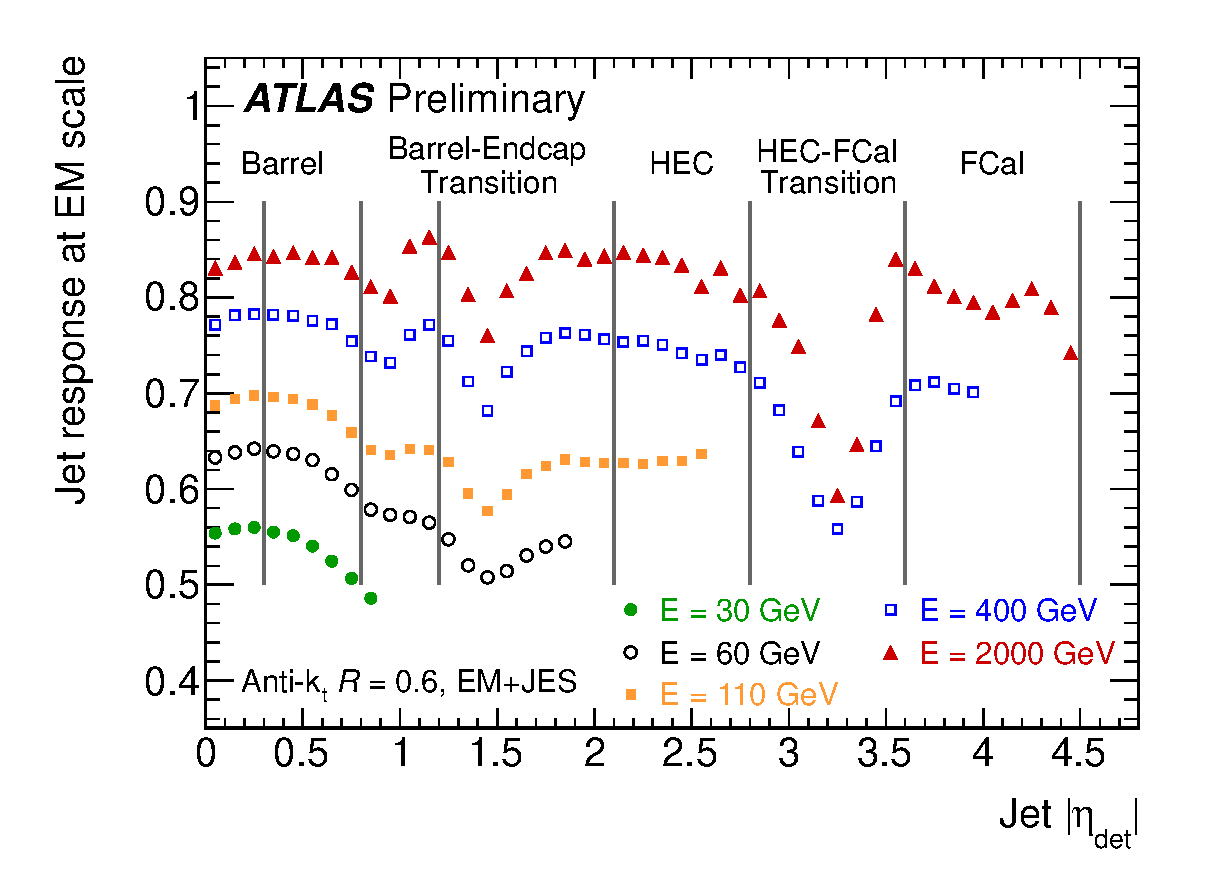
\includegraphics[width=0.495\textwidth]{ObjectReconstruction/Figures/JetCalibrationResponse.eps}
      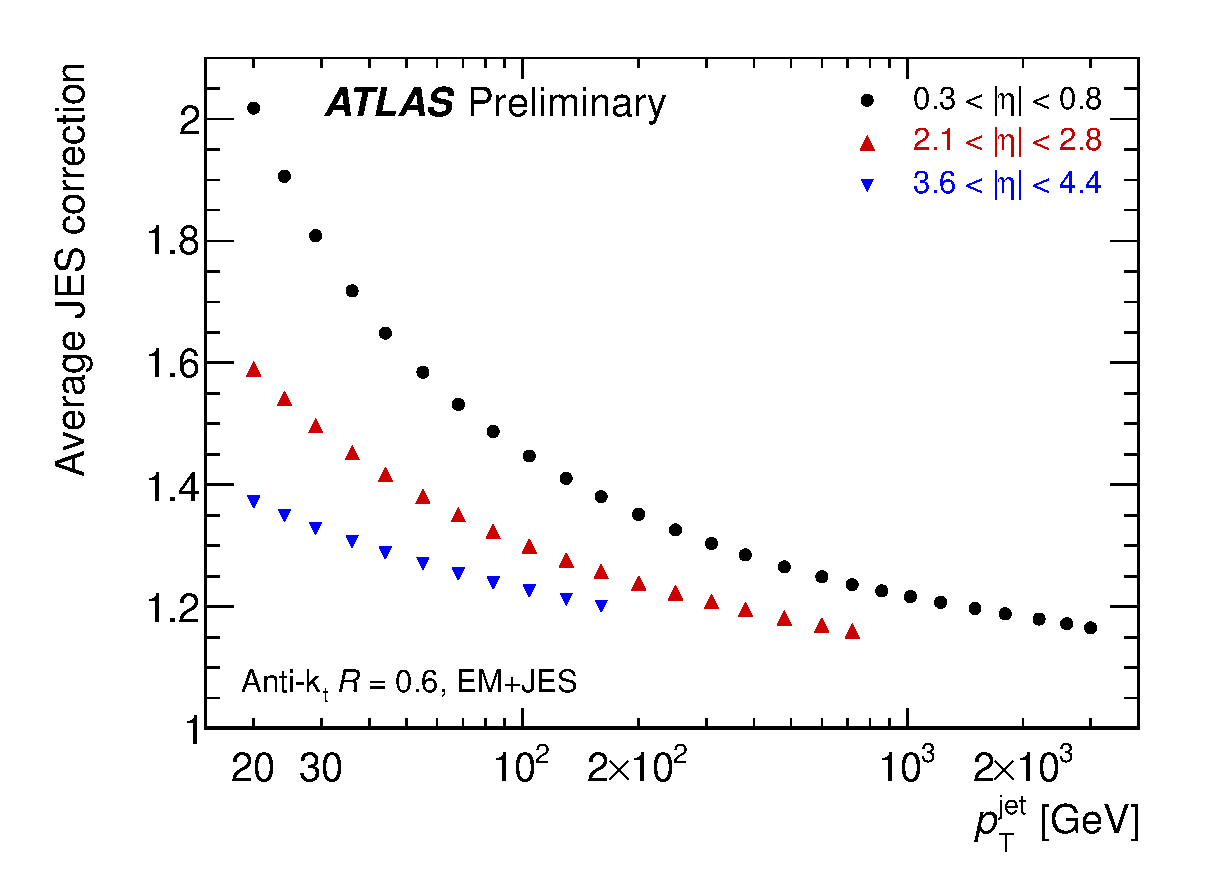
\includegraphics[width=0.495\textwidth]{ObjectReconstruction/Figures/JetCalibfig_EMJES_vs_pT_AntiKt6.eps}
    }
  \end{center}
  \caption[Average energy of jets formed from topoclusters calibrated at EM scale, and average jet energy scale correction as a function of the calibrated jet transverse momentum.]{Left: average energy of jets formed from topoclusters calibrated at EM scale with respect to the particle-level jet energy ($E_{\text{jet}}^{\text{EM}}/E_{\text{jet}}^{\text{truth}}$) as a function of the jet pseudorapidity before applying the correction for the event vertex shown separately for various jet energies \protect\cite{Aad:2011he}.
  Right: Average jet energy scale correction as a function of the calibrated jet transverse momentum for three representative $\eta^{\text{jet}}$-intervals obtained from the nominal MC simulation sample~\protect\cite{Aad:2011he}.
  }
  \label{fig:JetCalibrationResponse}
\end{figure}

The final jet energy scale correction that relates the measured calorimeter jet to the true jet energy is defined as $1/\mathcal{F}_{\text{calib}}(E_{\text{jet}}^{\text{EM(LCW)}})$, such that:

\begin{equation}
E_{\text{jet}}^{\text{EM+JES(LCW+JES)}} = \frac{E_{\text{jet}}^{\text{EM(LCW)}}}{\mathcal{F}_{\text{calib}}(E_{\text{jet}}^{\text{EM(LCW)}})|_{\eta}}.
\label{eq:JetJESCorrection}
\end{equation}

Figure \ref{fig:JetCalibrationResponse} (right) shows the jet energy scale correction as a function of the calibrated jet transverse momentum for three different $\eta$-intervals.
The values of the jet energy correction factors range from about 2.1 at low jet energies in the central region to less than 1.2 for high energy jets in the most forward region.


\subsubsection{Jet residual calibration}
    \label{subsubsec:JetResidualCalibration}

In the jet residual calibration, the data-to-MC differences are assessed using \emph{in-situ} techniques, which exploit the transverse momentum balance between a jet and well-measured photons, $Z$ bosons or jets.
This calibration is only applied to data, since it aims to restore the energy of the jets reconstructed in data to that from the Monte Carlo simulation\footnote{The reconstructed jets from the MC simulations are calibrated with the EM+JES or the LCW+JES scheme, which restores the reconstructed jet energy to that of the particle-level jet in the simulation, as shown in Section~\ref{subsubsec:JetEnergyCalibration}.}.
The jet energy once the residual calibration has been applied, $E_{\text{jet}}^{\text{data, in-situ}}$, is found to be:

\begin{equation}
E_{\text{jet}}^{\text{data, in-situ}} = \frac{E_{\text{jet}}^{\text{data}}}{\mathcal{C}(\pt^{\text{jet}}, \eta)},
\label{eq:JetInSituCorrection}
\end{equation}

\noindent where  $1 / \mathcal{C}(\pt^{\text{jet}}, \eta)$, the correction extracted from the jet in-situ calibrations, is defined as:

\begin{equation}
\mathcal{C}(\pt^{\text{jet}}, \eta) = \frac{\langle \pt^{\text{jet}} / \pt^{\text{ref}} \rangle_{\text{data}}}{\langle \pt^{\text{jet}} / \pt^{\text{ref}} \rangle_{\text{MC}}}\Bigg|_{\eta},
\label{eq:JetInSituCorrectionFactor}
\end{equation}

\noindent with $\langle \pt^{\text{jet}} / \pt^{\text{ref}} \rangle_{\text{data}}$ and $\langle \pt^{\text{jet}} / \pt^{\text{ref}} \rangle_{\text{MC}}$ being the ratio of the average jet response, measured in data and in the Monte Carlo simulation, respectively.

The residual jet calibration is computed following different strategies depending on whether the jet is contained in the central or in the forward regions of the detector.

In the central rapidity region, $|\eta_\text{det}|<1.2$, the jet energy can be calibrated as follows:

\begin{enumerate}
\item{\textbf{Jet energy calibration using $Z$-jet events: }}In events where one $Z$ boson is produced in association to only one jet, the jet recoils against the $Z$ boson ensuring approximate momentum balance between them in the transverse plane.
Ideally, the response of the jet in the calorimeters could be determined by using the $\pt$ of the $Z$ boson as the reference particle-level jet $\pt$.
However, uncertainties on the $Z$ boson decay products measurement, particles not included in the cone of the jet, additional parton radiation contributing to the recoil against the $Z$ boson or contributions from the underlying event prevent to use the measurement of $\langle\pt^{\text{jet}}/\pt^{\text{ref}}\rangle$ to estimate the jet response, but only to assess how well the MC simulation can reproduce the data.
Figure~\ref{fig:JetInSituMeasurements} (left) shows the mean $\pt$ balance measured in data and in a \pythia{} MC simulation, for EM+JES calibrated $\akt$ jets.
The $\pt$ balance, $\langle \pt^{\text{jet}} / \pt^{\text{ref}} \rangle$, ranges between 0.7 and 1 both in data and in the simulation, and it increases as the $\pt$ of the jet increases.
This figure also shows that the $\pt$ balance measured in the MC simulation is slightly higher compared to the measurement in data.
The advantage of the jet calibration using $Z$-jet events is the possibility of probing low-$\pt$ jets, which are difficult to reach with $\gamma$-jet events due to trigger thresholds and background contamination in that region.

\item{\textbf{Jet energy calibration using $\gamma$-jet events: }}The $\gamma$-jet events benefit from larger statistics for $\pt$ above 150~GeV compared to the $Z$-jet events.
Two in-situ techniques are used to probe the calorimeter response to jets recoiling the photons, for data and MC simulations.
On one hand, a technique based on the procedure used to determine the jet energy calibration using $Z$-jet events is followed, in which the highest $\pt$ jet is compared to the transverse momentum of the reference photon.
Alternatively, the missing transverse momentum projection fraction (MPF) technique \cite{Aad:2014bia} is used, in which the photon transverse momentum is balanced against the full hadronic recoil.

\item{\textbf{High-$\pt$ jet energy calibration: }}This technique is relevant for very high $\pt$ jets (at the TeV regime), where the calibrations extracted using the $Z$-jet and the $\gamma$-jet methods described above, are affected by statistical fluctuations.
Jets at very high $\pt$ are balanced against a recoil system of low $\pt$ jets, previously well calibrated using the $\gamma$-jet or the $Z$-jet balance.
\end{enumerate}

The final in-situ calibration obtained from the combination of these techniques is shown in Figure~\ref{fig:JetInSituMeasurements} (right), together with statistical uncertainties.
A general offset of about $-2\%$ is observed in the data-to-MC response ratios for jet transverse momenta below $\unit[100]{GeV}$.
The offset decreases to $-1\%$ at higher $\pt$ ($\pt \gtrsim \unit[200]{GeV}$).

\begin{figure}[!ht]
  \begin{center}
    \mbox{
      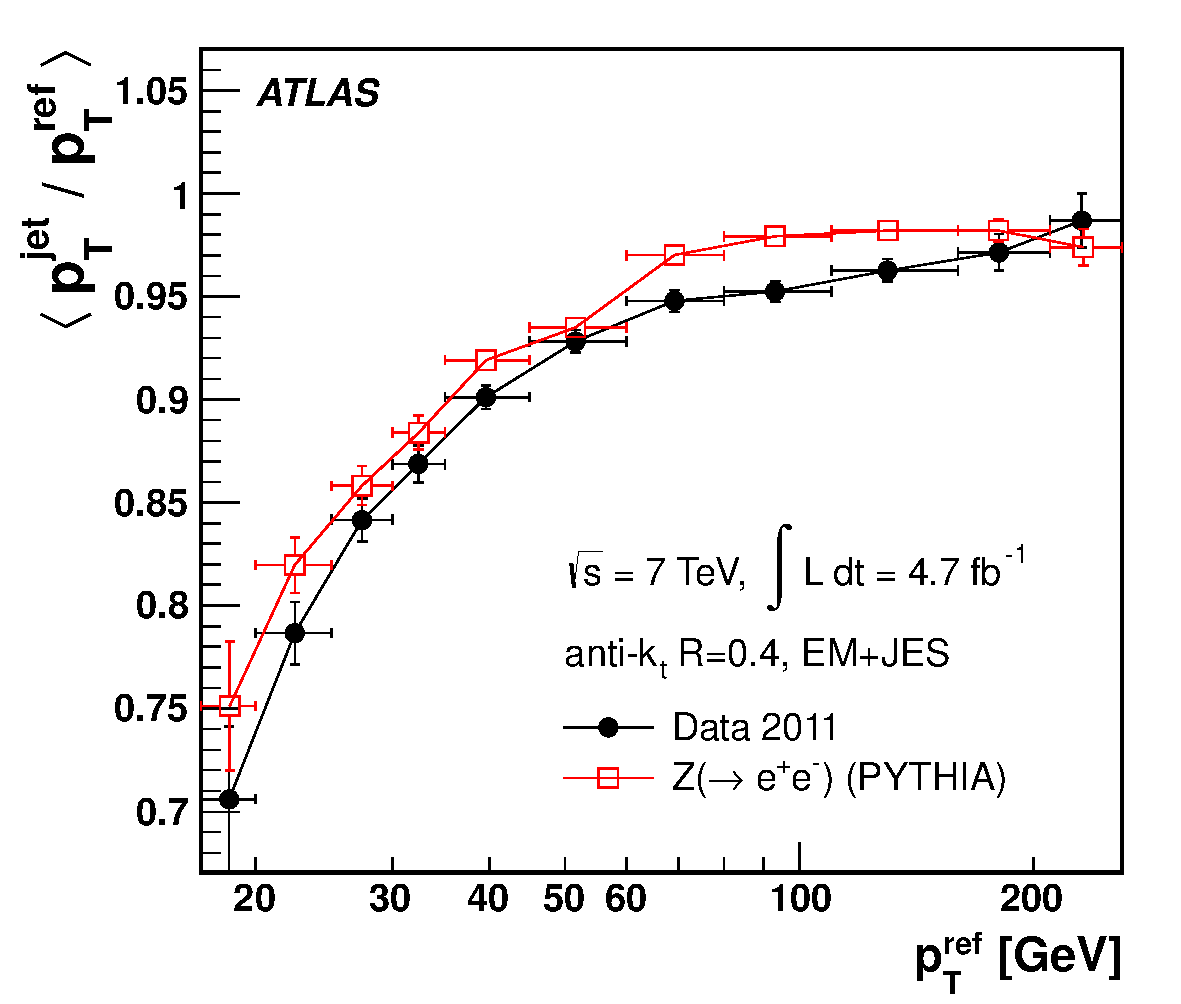
\includegraphics[width=0.495\textwidth]{ObjectReconstruction/Figures/Zjetfigures_balanceComparison_Jes_Akt4.pdf}
      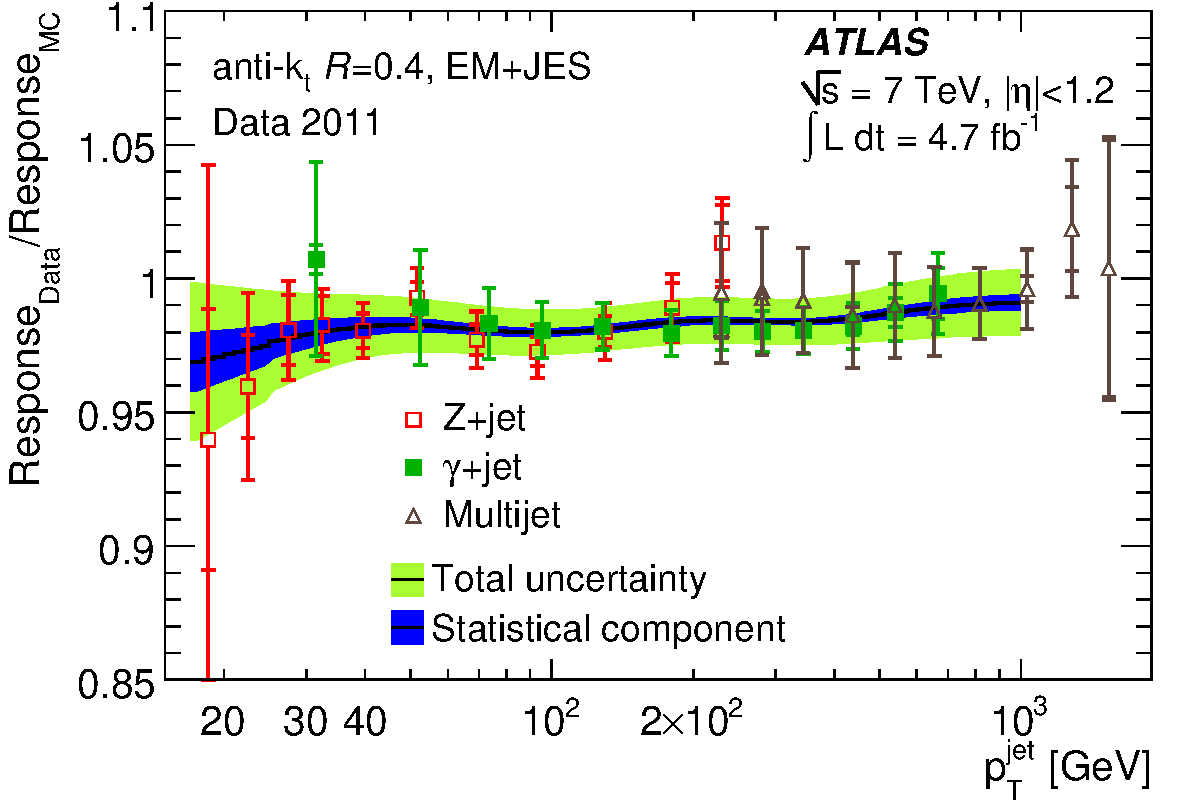
\includegraphics[width=0.495\textwidth]{ObjectReconstruction/Figures/responseRatioSmooth_TSpline2_EMJES_R4.pdf}
    }
  \end{center}
  \caption[Mean $\pt$ balance obtained in the data and with the \pythia{} simulation, and ratio of the average jet response measured in data to that measured in MC simulations.]{Mean $\pt$ balance obtained in the data and with the \pythia{} simulation, for $\akt$ jets with $R=0.4$ calibrated with the EM+JES scheme (left)~\cite{Aad:2014bia}. Ratio of the average jet response $\langle \pt^{\text{jet}} / \pt^{\text{ref}} \rangle$ measured in data to that measured in MC simulations for jets within $|\eta|<1.2$ as a function of the jet transverse momentum, $\pt^{\text{jet}}$, shown separately for the three in-situ techniques, used in the combined calibration (right)~\cite{Aad:2014bia}.}
  \label{fig:JetInSituMeasurements}
\end{figure}

In the forward rapidity region, $|\eta_\text{det}|>1.2$, the calibration can be performed by exploiting the transverse momentum balance in events with two jets at high transverse momentum. 
A jet in the forward region can be balanced against a well-calibrated jet in the central region, and therefore, the whole detector response can be equalized as a function of $\eta^{\text{jet}}$.
In addition to this simple approach, the matrix method described in Ref.~\cite{ATLAS:2011jea} is used, in which the $\eta$-intercalibration is estimated from jets in all regions (not only the central one).


\section{Missing transverse energy}
    \label{subsec:ETmissReco}

The missing transverse momentum, $\ptmiss$, is defined as the momentum imbalance in the plane transverse to the beam axis.
The vector momentum imbalance in the transverse plane is obtained from the negative vector sum of the momenta of all particles detected in a $\pp$ collision.
The $\ptmiss$ reconstruction includes contributions from energy deposits in the calorimeters and muons reconstructed in the muon spectrometer \cite{TheATLAScollaboration:2013oia}.
The two $\ptmiss$ components are calculated as:

\begin{equation}
p_{x(y)}^{\text{miss}} = p_{x(y)}^{\text{miss,calo}} + p_{x(y)}^{\text{miss},\mu}.
\label{eq:ETmissDef_All}
\end{equation}

The magnitude of this vector is the so-called missing transverse energy, $\met$.
The values of $\met$ and its azimutal coordinate $\phi^\text{miss}$ are defined as:

\begin{equation}
\begin{split}
\met = \sqrt{(p_{x}^{\text{miss}})^2 + (p_{y}^{\text{miss}})^2},\\
\phi^{\text{miss}} = \arctan{(p_{y}^{\text{miss}} / p_{x}^{\text{miss}})}.
\end{split}
\label{eq:ETmissDef_pol}
\end{equation}

The reconstruction of the calorimeter term of the $\ptmiss$ uses calorimeter cells calibrated according to the reconstructed high-$\pt$ physics object to which they are associated, in a chosen order: electrons, photons, hadronically decaying $\tau$-leptons, jets and muons.
Cells not associated with any such objects are also taken into account in the $\met$ calculation.
Once the cells are associated with objects as described above, the $\ptmiss$ calorimeter term is calculated as follows \cite{Aad:1379858} (the reason why the $p_{x(y)}^{\text{miss,calo},\mu}$ term is in between parenthesis will become clear below):

\begin{equation}
\begin{split}
p_{x(y)}^{\text{miss,calo}} = p_{x(y)}^{\text{miss},e} + p_{x(y)}^{\text{miss},\gamma} + p_{x(y)}^{\text{miss},\tau} + p_{x(y)}^{\text{miss,jets}} \\
    p_{x(y)}^{\text{miss,softjets}} + (p_{x(y)}^{\text{miss,calo},\mu}) + p_{x(y)}^{\text{miss,CellOut}}.
\end{split}
\label{eq:ETmissDef_Calo}
\end{equation}

Each of the terms in the previous equation is computed from the negative sum of calibrated cell energies inside the corresponding object, according to the following expression:

\begin{equation}
\begin{split}
p_{x}^{\text{miss,term}} = \sum_{i=1}^{N_{\text{cell}}^{\text{term}}}{p_i \sin{\theta_i}\cos{\phi_i}} \\
p_{y}^{\text{miss,term}} = \sum_{i=1}^{N_{\text{cell}}^{\text{term}}}{p_i \sin{\theta_i}\sin{\phi_i}}
\end{split}
\label{eq:ETmissDef_Split}
\end{equation}

\noindent where $p_i$, $\theta_i$ and $\phi_i$ are the energy, the polar angle and the azimutal angle respectively, and all the summations are performed on cells in the range $|\eta|<4.5$.

The different terms in Equation \ref{eq:ETmissDef_Calo} are described in the following:

\begin{itemize}

\item{$p_{x(y)}^{\text{miss},e}$ }is reconstructed from cells in clusters associated to electrons passing the ``medium'' identification criteria with $\pt>\unit[10]{GeV}$.

\item{$p_{x(y)}^{\text{miss},\gamma}$ }is also reconstructed from cells in clusters, associated with photons passing the ``tight'' identification criteria \cite{ATLAS:2012ana} with $\pt>\unit[10]{GeV}$ at the EM scale.

\item{$p_{x(y)}^{\text{miss},\tau}$ }is reconstructed from cluster cells associated to LCW calibrated $\tau$-jets reconstructed with the ``tight'' identification criteria \cite{TheATLAScollaboration:2013wha}, with $\pt>\unit[10]{GeV}$.

\item{$p_{x(y)}^{\text{miss,jets}}$ }is computed from cells in clusters associated to LCW calibrated jets with  $\pt>\unit[20]{GeV}$, reconstructed with the $\akt$ algorithm, and with the jet energy scale factor applied.

\item{$p_{x(y)}^{\text{miss,softjets}}$} is reconstructed from cells in clusters associated to LCW calibrated jets reconstructed with the $\akt$ algorithm (with $R=0.6$), with $\unit[7]{GeV}<\pt<\unit[20]{GeV}$.

\item{$p_{x(y)}^{\text{miss,calo},\mu}$} is the contribution originating from energy lost by muons in the calorimeter.
Its calibration will be discussed below.

\item{$p_{x(y)}^{\text{miss,CellOut}}$} is calculated from the cells in topoclusters with the LCW calibration and from reconstructed tracks with $\pt>\unit[400]{MeV}$  which are not included in the reconstructed objects.
 The tracks are added to recover the contribution from low-$\pt$ particles which do not reach the calorimeter or do not have enough energy to seed a topocluster.
They are also used to improve the determination of the momentum in the topoclusters, since the calibration and resolution of the low $\pt$ tracks is better compared to that of the topoclusters.

\end{itemize}

On the other hand, the $\ptmiss$ muon term (see Equation \ref{eq:ETmissDef_All}) from the momentum of muon tracks reconstructed with $|\eta|<2.7$:

\begin{equation}
p_{x(y)}^{\text{miss},\mu} = - \sum_{\text{muons}}{p_{x(y)}}^{\mu},
\label{eq:ETmissDef_Mu}
\end{equation}

\noindent where the summation effects all the selected muons.
In the central region, $|\eta|<2.5$, combined muons (reconstructed muons in the MS with a matched track in the ID, see Section \ref{sec:MuonReco}) are considered.
Instead, since the region $2.5<|\eta|<2.7$ lays outside the fiducial volume of the ID, there is no matched track requirement and the MS $\pt$ alone is used.

The muon term is calculated differently for isolated and non-isolated muons, where non-isolated muons are defined to be those within a distance $\Delta R < 0.3$ of a reconstructed jet in the event.
For isolated muons, the $\pt$ is determined from the combined measurement in the ID and MS, accounting for the energy that the muon deposits in the calorimeter.
Therefore, $p_{x(y)}^{\text{miss,calo},\mu}$ is not added to the calorimeter contribution (this is the reason why it appears in between parenthesis in Equation \ref{eq:ETmissDef_Calo}).
Instead, for non-isolated muons, the term $p_{x(y)}^{\text{miss,calo},\mu}$ has to be considered.

The systematic uncertainty on each individual term of the $\met$ can be evaluated from the propagation of the uncertainties of the reconstructed objects that are used to build it.
Only the contribution to the $\met$ scale and resolution uncertainties coming from the ``soft terms'' (softjets and CellOut terms) needs to be estimated with dedicated studies \cite{TheATLAScollaboration:2013oia}.
The overall systematic uncertainty on the $\met$ scale is then calculated by combining the uncertainties on each term.

As it will be discussed in Section~\ref{sec:ObjectDefinition}, a slightly modified definition of the $\met$ is used\footnote{The $\met$ collection in the analysis presented is called ``\texttt{MET\_Egamma10NoTau}''.} in the analysis presented in this Thesis.
The $\tau$-lepton term, $p_{x(y)}^{\text{miss},\tau}$, is omitted because in the analysis presented, $\tau$-leptons are not identified as such, but considered as jets.
Furthermore, the muon terms, $p_{x(y)}^{\text{miss,calo},\mu}$ and $p_{x(y)}^{\text{miss},\mu}$, are also omitted.
The reason for not considering them is related to the precise estimation of the most important irreducible background in the analysis, $\znn$, which will be explained in Chapter~\ref{chapter:MonojetAnalysis}.
